
\chapter{IMPLEMENTATION}

\section{Reference Implementation}

Alongside this publication, we provide a reference implementation of OnioNS. We utilize C++11, the Botan cryptographic library, the Standard Template Library's (STL) implementation of Mersenne Twister, and the libjsoncpp-dev library for JSON encoding. We develop in Linux Mint and compile for Ubuntu Vivid, Utopic, Trusty, and their derivatives. Our software is built on Canonical's Launchpad online build system and is available online on Github.

\section{Prototype Design}

We have developed an OnioNS prototype that implements the Record Generation and Domain Query protocols. In this initial prototype, we use a static server and a hidden service that we deployed at onions55e7yam27n.onion. We constructed a Record containing an association between ``example.tor'' and ``onions55e7yam27n.onion''. Next, we transmit this Record to the server over a Tor circuit. Finally, we modified Tor such that the following procedures occur client-side as illustrated in Figure \ref{fig:prototypeDiagram}:

\begin{enumerate}
	\item The user enters in ``example.tor'' into the Tor Browser.
	\item The Tor Browser sends ``example.tor'' to Tor's SOCKS port for resolution.
	\item The Tor client intercepts ``*.tor'', places the lookup in a wait state, and sends ``example.tor'' to the OnioNS client over a named pipe.
	\item The OnioNS client connects to the static OnioNS server over a Tor circuit and performs a Domain Query.
	\item The server responds with the Create Record containing ``example.tor''.
	\item The client writes ``onions55e7yam27n.onion'' to the Tor client over another named pipe.
	\item The Tor client resumes the lookup and rewrites the original ``example.tor'' lookup with ``onions55e7yam27n.onion''.
	\item The Tor client contacts the OnioNS hidden service and passes the webpage to the Tor Browser.
	\item The Tor Browser displays the website contents and preserves the ``example.tor'' domain name.
\end{enumerate}

\begin{figure}[htbp]
	\centering
	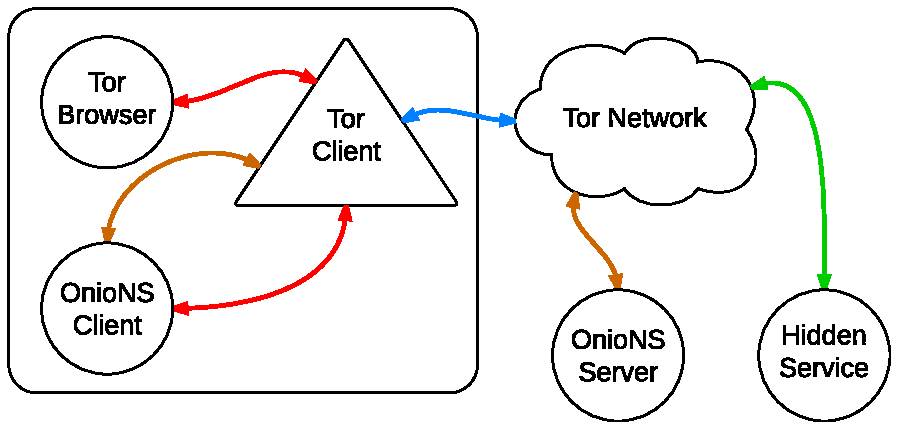
\includegraphics[width=0.6\textwidth]{images/LucidCharts/OnioNS_Prototype.pdf}
	\caption{The overview of our OnioNS prototype. The Tor Browser passes an unknown .tor domain to the OnioNS through the Tor software (red) which resolves the domain anonymously over a Tor circuit (orange) to a remote resolver. Finally, the Tor software contacts the hidden service in the traditional way. (green) The Tor Browser communicates to the Tor client over its SOCKS port, while the OnioNS client communicates over named pipes (red) and Tor's SOCKS port (orange).}
	\label{fig:prototypeDiagram}
\end{figure}

Tor performs asynchronously here; it must place the lookup on hold, free its event loop to avoid a deadlock, and asynchronously resume the lookup once it receives the response. From the user's perspective, the content of \url{http://onions55e7yam27n.onion} loads transparently under the \url{http://example.tor} URL.

\subsection{Challenges}

We encountered two significant challenges while implementing the prototype. 

Our first modification to the Tor software used blocking I/O for communication with the OnioNS client. This caused Tor's event loop to pause while the OnioNS was resolving the domain name. When the OnioNS client attempted to use Tor to construct a circuit to the OnioNS server, Tor could not respond as it was waiting on I/O. This resulted in an unresolvable deadlock. After collaboration with several Tor developers we migrated our Tor modification to libevent, a software library that enables asynchronous event. Libevent is heavily used throughout Tor, Google Chrome, ntpd, and other software. Libevent enabled the OnioNS client to communicate over Tor, communicate with the remote OnioNS resolver, and return the hidden service address to Tor. Libevent then fired a callback method to contact the hidden service.

Our second challenge was telling Tor to place the resolution of the domain on hold. Previously, Tor would attempt to interpret the .tor domain and fail the lookup almost instantaneously. To resolve this, we placed the resolution in a waiting state. Then when OnioNS resolved the domain, our Libevent callback resumed the lookup, passed in the initial state, and allowed the lookup to continue as if a hidden service address had been requested in the first place. This allowed the Tor Browser to view the destination hidden service under a .tor domain name.

\subsection{Performance}

We conducted several performance measurements for the Record Generation and Domain Query protocols. Our experiment involves two machines, A and B. Machine A has an Intel Core2 Quad Q9000 (Penryn architecture) @ 2.00 GHz CPU from late 2008 and Machine B has an Intel i7-2600K (Sandy Bridge architecture) @ 4.3 GHz CPU from 2011. We chose machines with this hardware in order to represent low-end and medium-end consumer-grade computers, respectively. To minimize latency on our end, both machines were hosted on 1 Gbits connections at Utah State University. We hosted our hidden service and TCP server on Machine B. Then on Machine A, we measured the time required to connect to our hidden service over OnioNS and over the more direct hidden service protocol.

We selected the parameters of scrypt such that it consumed 128 MB of RAM during operation. We consider this an affordable amount of RAM for low-end consumer-grade computers. We created a multi-threaded implementation of the Record Generation protocol and used all eight virtual CPU cores on Machine B to generate our Record. As expected, our RAM consumption scaled linearly with the number of scrypt instances executed in parallel; we observed approximately 1 GB of RAM consumption during Record Generation. We set the difficulty of the Create Record such that the Record Generation protocol took only a few minutes on average to conduct, but in the future we may change it so that the protocol takes several hours instead.

\subsubsection{Processing Time}

We measured the CPU wall time required for different parts of client-side protocols. We measured how long it takes the client to build a Record from a JSON-formatted textual string, which involves parsing and assembly of the various fields; the time to check the proof-of-work \emph{PoW}, and the time to check the \emph{recordSig} digital signature.

\renewcommand{\arraystretch}{1}
\begin{center}
    \begin{tabular}{ | c | c | c | c |}
    \hline
    \textbf{Description} & \textbf{A Time (ms)} & \textbf{B Time (ms)} & \textbf{Samples} \\
    \hline
    Parsing JSON into a Record & 0.052 & 0.0238 & 100 \\ \hline
	Scrypt check & 896.369 & 589.926 & 25 \\ \hline
	Check of $ S_{d}(m, r) $ RSA signature & 0.06304 & 0.0267 & 200 \\
	\hline
    \end{tabular}
\end{center}

Machine B, as expected, performed much faster than Machine A at all of these tasks. Parsing and signature checks both took trivial time, though the total time was dominated by the single iteration of scrypt. Record Validation protocol is single threaded and consumes 128 MB of RAM due to scrypt.

\subsubsection{Latency}

We compared the load latency between an OnioNS domain name with a traditional hidden service address. Our tests measured the time between when a user entered in ``example.tor'' into the Tor Browser to the time when the browser first began to load our hidden service webpage. We also tested \url{http://onions55e7yam27n.onion}, the destination of ``example.tor''. We performed our experiment 15 times with a different client-side Tor circuit for each by restarting Tor at each iteration. To prevent browser-side caching, we restarted the Tor Browser between tests as well. 

\renewcommand{\arraystretch}{1}
\begin{center}
    \begin{tabular}{ | c | c | c | c |}
    \hline
    \textbf{Lookup} & \textbf{Fastest Time} & \textbf{Slowest Time} & \textbf{Mean Time} \\
    \hline
    .tor & 6.1 & 8.5 & 7.1 \\ \hline
	.onion & 9.3 & 12.2 & 10.2 \\
	\hline
    \end{tabular}
\end{center}

The latency is circuit-dependent and heavily depends on the speed of each Tor router and the distance between them. To avoid the latency cost whenever possible, we implemented a DNS cache into the OnioNS client-side software to allow subsequent queries to be resolved locally, avoiding unnecessary remote lookups.
